\documentclass{beamer}
\usepackage{../common_slides}
\usepackage{tikz}
\usepackage{tikz-qtree}
\usepackage{pdfpages}


\usetikzlibrary{bayesnet,matrix}
% \usepackage{enumitem}

\title{Machine Translation 1}
\date{}
\author{CS 287}

\begin{document}
\begin{frame}
  \titlepage
\end{frame}


\begin{frame}{Review: Conditional Random Field (Lafferty et al, 2001)}
  \begin{itemize}
  \item Model consists of unnormalized weights 

    \[\log \hat{\boldy}(c_{i-1})_{c_i} = feat(\boldx, c_{i-1}) \boldW + \boldb\]
    
  \item Out of log space, 

    \[ \hat{\boldy}(c_{i-1})_{c_i} = \exp(feat(\boldx, c_{i-1}) \boldW + \boldb)\]

    

  \item Score of the sequence, (same as last few classes)
    
    \[ f(\boldx, c_{1:n}) = \sum_{i=1}^n \log \hat{y}(c_{i-1})_{c_{i}} \] 
    % \[ p(\boldy  | \boldx ) =  \softmax\ \mathrm { over\ all\ sequences}    \] 

  \item Objective is based on global NLL of this sequence distribution
    \[\boldz_{c_{1:n}} =  f(\boldx, c_{1:n})    \] 

  \end{itemize}
\end{frame}

 \begin{frame}{Review: Computing the Softmax}
   Want to compute:
   \[ p(\boldy=\delta(c_{1:n}) | \boldx) = \frac{\displaystyle \prod_{i=1}^n \hat{\boldy}(c_{i-1})_{c_i}} {\displaystyle  \sum_{c'_{1:n}} \prod_{i=1}^n \hat{\boldy}(c'_{i-1})_{c'_i} }\] 

   \begin{itemize}
   \item $\displaystyle \prod_{i=1}^n \hat{\boldy}(c_{i-1})_{c_i}$; easy to compute
     \air 
   \item $\displaystyle \sum_{c'_{1:n}} \prod_{i=1}^n \hat{\boldy}(c'_{i-1})_{c'_i}$; can use forward algorithm.
   \end{itemize}j

   Softmax goes from $O(|\mcC|^n)$ to $O(|\mcC|^2)$.  
 \end{frame}

 \begin{frame}{Review: Final Gradients}
   \begin{eqnarray*}
    \frac{\partial L}{\partial \log \hat{y}_i(c'_{i-1})_{c'_{i}}} &=&
    \sum_{d_{1:n}} \frac{\partial z_{d_{1:n}} }{\partial \log \hat{y}_i(c'_{i-2})_{c'_{i}}} \frac{\partial L } {\partial z_{d_{1:n}}}  \\
     &=& \sum_{c'_{1:i-2}, c'_{i+1:n}}  \frac{\partial L }{\partial z_{c'_{1:n}}}  \\
    &=& p(\boldy_{i-1} = c'_{i-1}, \boldy_{i} = c'_{i}  | \boldx) - \indicator(c'_{i-1} = c_{i-1} \land c'_{i} = c_i)
   \end{eqnarray*}

   \begin{itemize}
   \item First term, marginals of the CRF. 

     \air 

   \item Second term, indicator of whether edge is in gold.
   \end{itemize}
 \end{frame}


\begin{frame}{Quiz: CRF}
  Note: Nothing in our definition of CRFs relied on $\boldy_i$ to align
  with $\boldx_i$ (conditioned on full sequence). 

  For this quiz, imagine we have an input sequence $\boldx$, and we want to 
  find the optimal output sequence $\boldy$ but we do not fix $n < N$. For instance 
  finding the best word segmentation of an unsegmented input $\boldx$. 

  \begin{itemize}
  \item How would you find \[ \argmax_{n, c_{1:n}} f(\boldx, c_{1,n}) ?\]

  \item How would you train \[ f(\boldx, c_{1,n}; \theta) ?\] 
  \end{itemize}
\end{frame}

{
\setbeamercolor{background canvas}{bg=}
\includepdf[pages=3]{jobslides.pdf}
}

\begin{frame}{Machine Translation }
  \begin{center}
    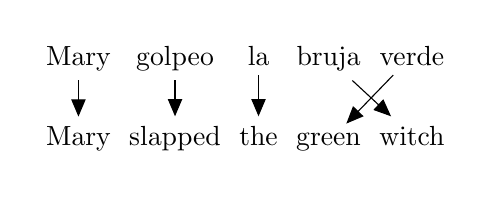
\begin{tikzpicture}
    \matrix(dict)[matrix of nodes, ampersand replacement=\&]{
      Mary \& golpeo \& la \& bruja \& verde \\
      ~\\
      ~\\
      Mary \& slapped \& the \& green \& witch  \\ };
    \path[draw, ->] (dict-1-1) -> (dict-4-1);
    \path[draw, ->] (dict-1-2) -> (dict-4-2);
    \path[draw, ->] (dict-1-3) -> (dict-4-3);
    \path[draw, ->] (dict-1-4) -> (dict-4-5);
    \path[draw, ->] (dict-1-5) -> (dict-4-4);
  \end{tikzpicture}
  \end{center}
\end{frame}

\begin{frame}{Today's Lecture}
  \begin{itemize}
  \item History of Translation
    \air 

  \item Statistical Machine Translation 
    \air 

  \item Simplified Translation Models
    \air
 
  \item Search for Translation
  \end{itemize}
  \air 

  Next Class: Neural Machine Translation
\end{frame}

\section{History of Automatic Translation}

\begin{frame}{Early Ideas of Translation}
  \begin{quote}
    . . . one naturally wonders if the problem of translation could
conceivably be treated as a problem in cryptography. When I
look at an article in Russian, I say: “This is really written in
English, but it has been coded in some strange symbols. I will
now proceed to decode.”
  \end{quote}
  Letter from Warren Weaver to Norbert Weiner, 1947
\end{frame}

\begin{frame}{Shannon's Noisy Channel (Shannon, 1948)}
  \begin{center}
    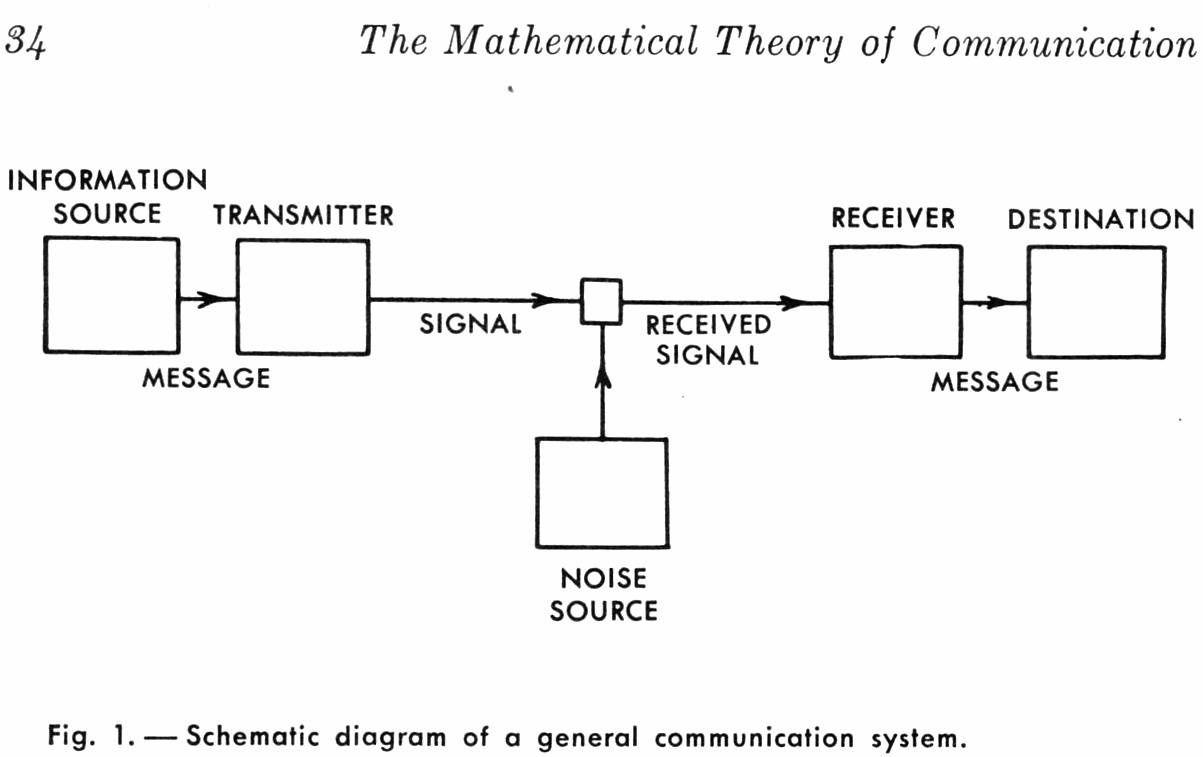
\includegraphics[width=10cm]{shannonchannel}
  \end{center}
\end{frame}

\begin{frame}{Noisy Channel}
  \begin{itemize}
  \item Method provides a basis for thinking about translation.
    \air 
  \item However how do you actually learn what the encoder/decoder are?
    \air 

  \item We will focus on learning from data. 
  \end{itemize}
\end{frame}

\begin{frame}
  \begin{small}
  \begin{quote}
    The 35th Parliament having been dissolved by proclamation on
    Sunday, April 27, 1997, and writs having been issued and returned,
    a new Parliament was summoned to meet for the dispatch of business
    on Monday, September 22, 1997, and did accordingly meet on that
    day.  Monday, September 22, 1997 This being the day on which
    Parliament was convoked by proclamation of His Excellency the
    Governor General of Canada for the dispatch of business, and the
    members of the House being assembled: Robert Marleau, Esquire,
    Clerk of the House of Commons, read to the House a letter from the
    Administrative Secretary to the Governor General informing him
    that the Right Honourable Antonio Lamer, in his capacity as Deputy
    Governor General, would proceed to the Senate chamber to open the
    first session of the 36th Parliament of Canada on Monday,
    September 22 at Ottawa.  A message was delivered by the Gentleman
    Usher of the Black Rod as follows: Members of the House of
    Commons: 
  \end{quote}
  \end{small}
\end{frame}

\begin{frame}
  \begin{small}
  \begin{quote}
    La trente-cinquième législature ayant été prorogée et les Chambres dissoutes par proclamation le dimanche 27 avril 1997, puis les brefs ayant été émis et rapportés, les nouvelles Chambres ont été convoquées pour l'expédition des affaires le lundi 22 septembre 1997 et, en conséquence, se sont réunies le jour dit.  
Le lundi 22 septembre 1997.  
Le Parlement ayant été convoqué pour aujourd'hui, par proclamation de Son Excellence le Gouverneur général du Canada pour l'expédition des affaires, et les députés étant réunis: 
M. Robert Marleau, greffier de la Chambre, donne lecture d'une lettre du directeur administratif du Gouverneur général annonçant que le très honorable Antonio Lamer, à titre de suppléant du Gouverneur général, se rendra à la salle du Sénat le lundi 22 septembre 1997, à Ottawa, pour ouvrir la première session de la trente-sixième législature.  
Le gentilhomme huissier de la verge noire apporte le message suivant: 
Membres de la Chambre des communes: 

  \end{quote}
  \end{small}
\end{frame}

\begin{frame}{Hansard's Corpus}
  
\end{frame}

\begin{frame}{Statistical Machine Translation}
  \begin{center}
    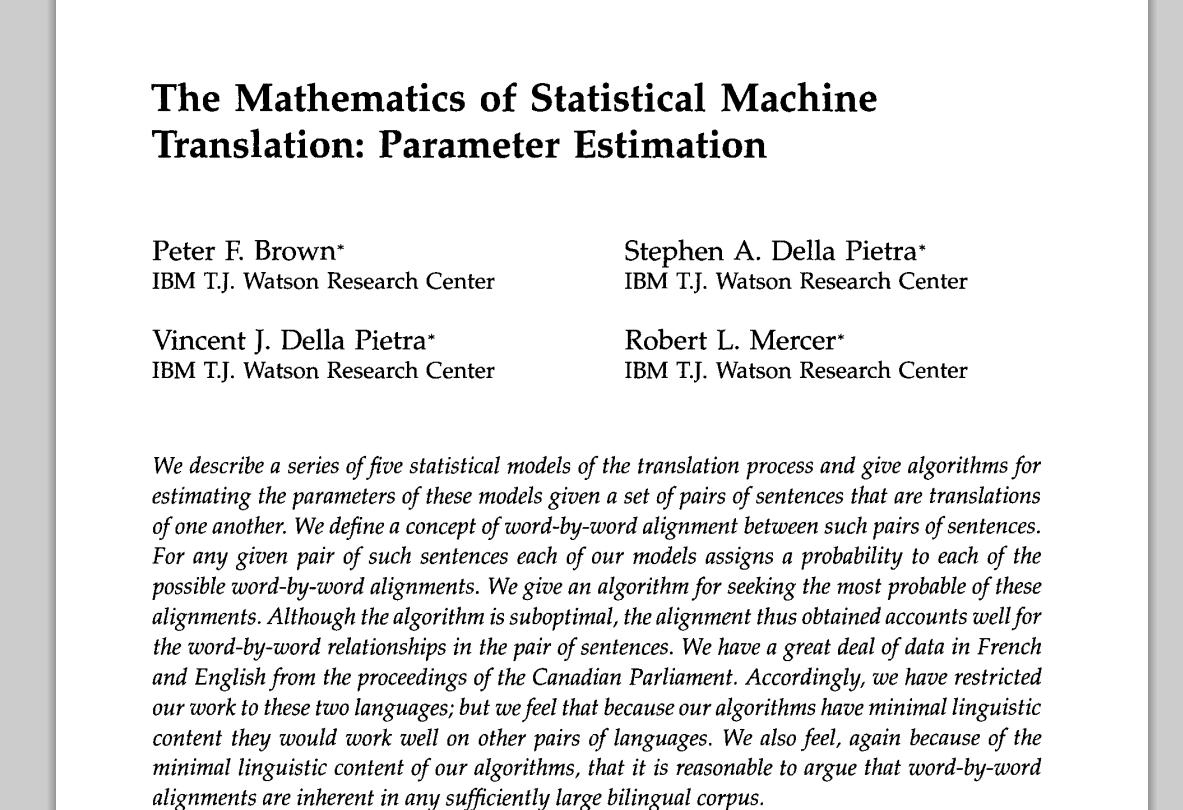
\includegraphics[width=9cm]{mathofmt}
  \end{center}
\end{frame}


{
\setbeamercolor{background canvas}{bg=}
\includepdf[pages=65]{jobslides.pdf}
}

\begin{frame}{Evaluation}
  How do you evaluate machine translation output?
  
  \begin{itemize}
  \item Model produces one output, compared to several references.
    \air
  \item Want a corpus-wide metric (short sentences count less)
  \end{itemize}

\end{frame}

\begin{frame}{BLEU (Papineni et al, 2002)}
    Main metric: BLEU (bilingual evaluation understudy)

  \begin{itemize}
  \item Calculate the \textit{precision} of unigrams, bigrams, trigrams, 4-grams
    \air 
  \item Take the geometric mean of corpus precision scores
    \air 
  \item Use length penalty to ensure appropriately long translations 
  \end{itemize}

  \[ \log BLEU = \min(0, 1 - \frac{\mathrm{ref\ len}}{\mathrm{cand\ len}}) + \mathrm{\ mean \ of \ log \ precisions} \] 

\end{frame}


\begin{frame}{BLEU}
  \begin{center}
    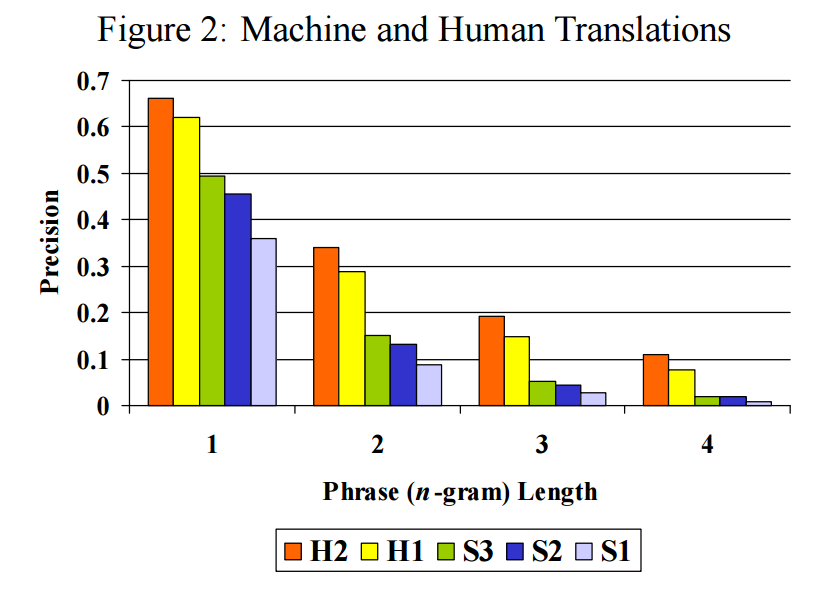
\includegraphics[width=7cm]{bleulen}
  \end{center}
\end{frame}
% \begin{frame}
%   Slapped the green witch.
% \end{frame}

% \begin{frame}{Shannon Noisy Channel Model}
  
% \end{frame}

% \begin{frame}{Encoder-Decoder}
%   \begin{itemize}
%   \item Idea
%   \item Encoder
%   \item Decoder 
%   \end{itemize}
% \end{frame}

\section{Noisy-Channel Models}

\begin{frame}{Noisy-Channel Model}
  Notation: Source words and target words
  \begin{itemize}
  \item $\boldx  = [ w^s_1\ w^s_2\ w^s_3\ldots w^s_n $] 
  \item $\boldy =  [w^t_1\ w^t_2\ w^t_3\ldots w^t_n $] 
  \end{itemize}

  \[ p(\boldy | \boldx) \propto p(\boldy) p(\boldx | \boldy) \] 


  Translation is reversing noisy channel-process,
  \begin{itemize}
  \item $p(\boldy)$ - prob generating target sentence
  \item $p(\boldx | \boldy)$ - prob of converting to source language
  \end{itemize}
\end{frame}

\begin{frame}{Translation}
  How do we model these two distributions?:
  \air
  
  \begin{enumerate}
  \item Language Model ($p(\boldy)$) 
    \air 

  \item Translation Model ($p(\boldx | \boldy)$) 
  \end{enumerate}
\end{frame}


\begin{frame}{One-to-One In-Order Translation}
  \textbf{Thought Experiment 1:}
  What if the two languages just involved word to word 
  translation?

  \begin{center}
    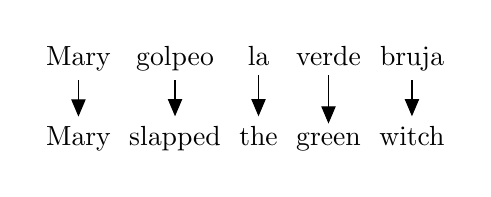
\begin{tikzpicture}
    \matrix(dict)[matrix of nodes, ampersand replacement=\&]{
      Mary \& golpeo \& la \& verde  \& bruja  \\
      ~\\
      ~\\
      Mary \& slapped \& the \& green \& witch  \\ };
    \path[draw, ->] (dict-1-1) -> (dict-4-1);
    \path[draw, ->] (dict-1-2) -> (dict-4-2);
    \path[draw, ->] (dict-1-3) -> (dict-4-3);
    \path[draw, ->] (dict-1-4) -> (dict-4-4);
    \path[draw, ->] (dict-1-5) -> (dict-4-5);
  \end{tikzpicture}
  \end{center}
  
  Notation: Source words and target words
  \begin{itemize}
  \item $\boldx  = [ w^s_1\ w^s_2\ w^s_3\ldots w^s_n $] 
  \item $\boldy =  [w^t_1\ w^t_2\ w^t_3\ldots w^t_n $] 
  \end{itemize}
\end{frame}


\begin{frame}{Simple One-to-One Model}
  \begin{enumerate}
  \item Language Model; words depend on previous word
    \[ p(\boldy) = \prod_{i=1}^n p(\boldy_i | \boldy_{i-1})  \] 
    \air 

  \item Translation Model; source word depends on current position
    \[ p(\boldx | \boldy) = \prod_{i=1}^n p(\boldx_i | \boldx_{i-1})  \] 
  \end{enumerate}

  What model is this?
\end{frame}


\begin{frame}{Answer: Hidden Markov Model}
  \begin{center}  
    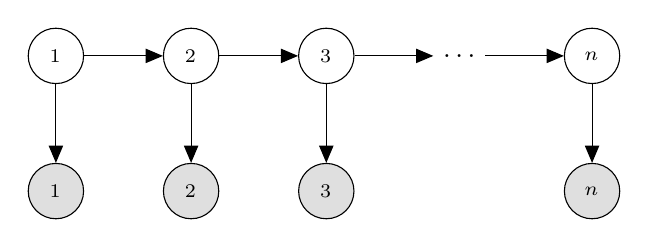
\begin{tikzpicture}
      \node (Ea) [obs] {$\boldx_1$}; 
      \node (Xa) [latent,above =of Ea] {$\boldy_1$};
      
      \node (Eb) [obs, right = of Ea ] {$\boldx_2$}; 
      \node (Xb) [latent,above =of Eb] {$\boldy_2$}; 
      
      \node (Ec) [obs, right = of Eb] {$\boldx_3$}; 
      \node (Xc) [latent,above =of Ec] {$\boldy_3$}; 
      \node (Xd) [right =of Xc] {$\ldots$}; 
      \node (Xe) [latent,right =of Xd] {$\boldy_n$}; 
    \node (Ee) [obs,below =of Xe] {$\boldx_n$}; 
    
    \edge {Xa} {Xb} ; %
    \edge {Xb} {Xc} ; %
    \edge {Xa} {Ea} ; %
    \edge {Xb} {Eb} ; %
    \edge {Xc} {Ec} ; %
    \edge {Xc} {Xd} ; %
    \edge {Xd} {Xe} ; %
    \edge {Xe} {Ee} ; %
  \end{tikzpicture}
\end{center}  
\end{frame}




% \begin{frame}{Language Model}
%   \[ p(\boldy) = \prod_{i=1} p(w^{t}_i | w^{t}_{i-n+1}, \ldots, w^{t}_{i-1})  \] 
% \end{frame}


\begin{frame}{How might you estimate this?}  
  \begin{itemize}
  \item Language model. Standard forms of Markov model estimation
    (Could use n-gram model or NNLM )
  \item Translation Model
  \[ p(\boldx_i | \boldy_i)  \]


  \[ p(\boldx_i | \boldy_i )\] 
  Assume we have many examples of language. 
  \end{itemize}

  Why estimate separate LM and TM?
\end{frame}


\begin{frame}{Conditional Random Field}
  \begin{itemize}
  \item Could also utilize CRF model. 
    \air 
  \item Finding the optimal translation (as in quiz)
    \[ \argmax_{w^t_{1:n}} f(\boldx, w^t_{1:n}) \] 
    
    \air
  \item What would be benefits? Downsides?
  \end{itemize}

\end{frame}


\section{True Translation}

\begin{frame}{Out-of-Order One-to-One Translation}
  \textbf{Thought Experiment 2:}
  Assume 1-to-1 still but allow any order. 

  \begin{center}
    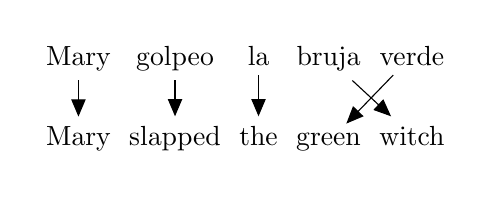
\begin{tikzpicture}
    \matrix(dict)[matrix of nodes, ampersand replacement=\&]{
      Mary \& golpeo \& la \& bruja \& verde \\
      ~\\
      ~\\
      Mary \& slapped \& the \& green \& witch  \\ };
    \path[draw, ->] (dict-1-1) -> (dict-4-1);
    \path[draw, ->] (dict-1-2) -> (dict-4-2);
    \path[draw, ->] (dict-1-3) -> (dict-4-3);
    \path[draw, ->] (dict-1-4) -> (dict-4-5);
    \path[draw, ->] (dict-1-5) -> (dict-4-4);
  \end{tikzpicture}
  \end{center}

\end{frame}



% \begin{frame}
%   Scores 
%   $p(\boldy) p(\boldx | \boldy)  $ 
% \end{frame}

\begin{frame}{Alignment}
  \begin{itemize}
  \item $\bolda$; alignment mapping each target word to a source word
  \item Assuming one-to-one
  \end{itemize}


  \begin{center}
    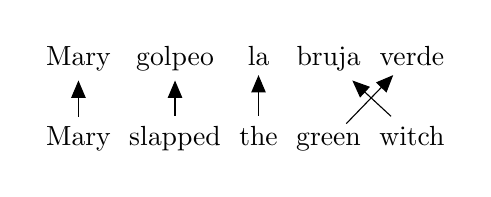
\begin{tikzpicture}
    \matrix(dict)[matrix of nodes, ampersand replacement=\&]{
      Mary \& golpeo \& la \& bruja \& verde \\
      ~\\
      ~\\
      Mary \& slapped \& the \& green \& witch  \\ };
    \path[draw, <-] (dict-1-1) -> (dict-4-1);
    \path[draw, <-] (dict-1-2) -> (dict-4-2);
    \path[draw, <-] (dict-1-3) -> (dict-4-3);
    \path[draw, <-] (dict-1-4) -> (dict-4-5);
    \path[draw, <-] (dict-1-5) -> (dict-4-4);
  \end{tikzpicture}
  \end{center}
  \begin{center}
  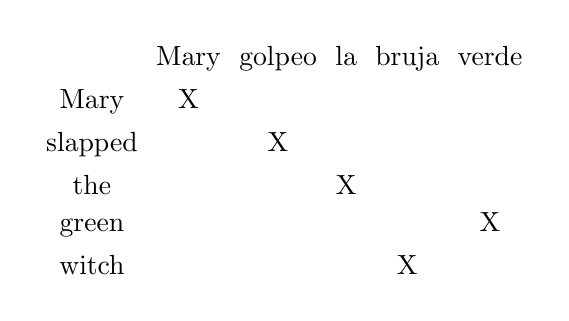
\begin{tikzpicture}
    \matrix(dict)[matrix of nodes, ampersand replacement=\&]{
      \ \& Mary \& golpeo \& la \& bruja \& verde \\
      Mary \& X \&  \&  \&  \&  \\
      slapped \&  \& X \&  \&  \&  \\
      the \&  \&  \&  X\&  \&  \\
      green \&  \&  \&  \&  \& X \\
      witch \&  \&  \&  \& X  \&  \\
    };
    \end{tikzpicture}
  \end{center}
\end{frame}

\begin{frame}{Alignment Model}
  \begin{itemize}
  \item Probability of alignment order,
    \[ p(\bolda | \boldy) \]

    \air 
  \item Models typically look at movement and past alignment choices,
    \[p(\bolda= c_{1:n} | \boldy) = \prod_{i=1}^n p(a_i=c_i | a_{i-1}=c_{i-1}, i) \]
    \air

  \item But with constraint that all words used exactly once.

    \air 

  \item (Vastly Simplified version, many different approaches)

  \end{itemize}
\end{frame}

\begin{frame}{Using Alignments}
  \[ p(\boldy | \boldx) \propto \sum_{\bolda} p(\boldy) p(\bolda | \boldy) p(\boldx |  \bolda, \boldy)  \]  

  With alignment,
  \[ p(\boldx |  \bolda, \boldy)  = \prod_{i=1}^n p(\boldx_{a_i} | \boldy_i) \] 

  \air 

  Sum-over-alignment approximated with a max-over-alignment,

  \[ \argmax_{j, w^t_{1:n}} \prod_{i=1}^n p(\boldx_{a_i} | \boldy_i=w^t_i) p(\boldy_i=w^t_i | \boldy_{i-1}=w^t_{i-1}) p(a_i = c_i | a_{i-1}=c_{i-1}, i)   \]  

\end{frame}

\begin{frame}{Example: Possible Alignment}
\begin{center}  
  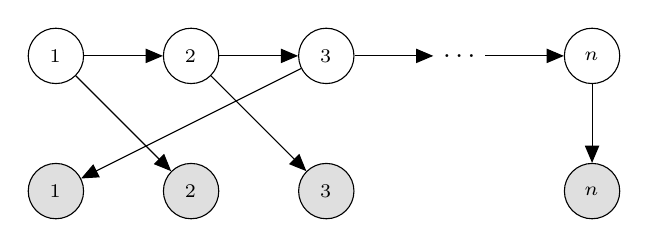
\begin{tikzpicture}
    \node (Ea) [obs] {$\boldx_1$}; 
    \node (Xa) [latent,above =of Ea] {$\boldy_1$}; 

    \node (Eb) [obs, right = of Ea ] {$\boldx_2$}; 
    \node (Xb) [latent,above =of Eb] {$\boldy_2$}; 

    \node (Ec) [obs, right = of Eb] {$\boldx_3$}; 
    \node (Xc) [latent,above =of Ec] {$\boldy_3$}; 
    \node (Xd) [right =of Xc] {$\ldots$}; 
    \node (Xe) [latent,right =of Xd] {$\boldy_n$}; 
    \node (Ee) [obs,below =of Xe] {$\boldx_n$}; 

    \edge {Xa} {Xb} ; %
    \edge {Xb} {Xc} ; %
    \edge {Xa} {Eb} ; %
    \edge {Xb} {Ec} ; %
    \edge {Xc} {Ea} ; %
    \edge {Xc} {Xd} ; %
    \edge {Xd} {Xe} ; %
    \edge {Xe} {Ee} ; %
  \end{tikzpicture}
\end{center}  
\end{frame}



\begin{frame}{Decoding Quiz}
  We have seen two translation models, one with a fixed order and 
  one where we had alignment as a latent variable. 

  \air 
  \begin{itemize}
  \item What is the complexity in the fixed-order case?

  \begin{center}  
    \scalebox{0.5}{
    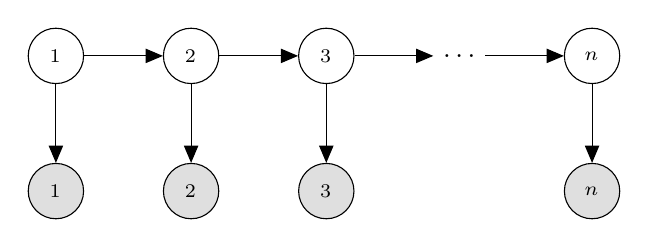
\begin{tikzpicture}
      \node (Ea) [obs] {$\boldx_1$}; 
      \node (Xa) [latent,above =of Ea] {$\boldy_1$};
      
      \node (Eb) [obs, right = of Ea ] {$\boldx_2$}; 
      \node (Xb) [latent,above =of Eb] {$\boldy_2$}; 
      
      \node (Ec) [obs, right = of Eb] {$\boldx_3$}; 
      \node (Xc) [latent,above =of Ec] {$\boldy_3$}; 
      \node (Xd) [right =of Xc] {$\ldots$}; 
      \node (Xe) [latent,right =of Xd] {$\boldy_n$}; 
    \node (Ee) [obs,below =of Xe] {$\boldx_n$}; 
    
    \edge {Xa} {Xb} ; %
    \edge {Xb} {Xc} ; %
    \edge {Xa} {Ea} ; %
    \edge {Xb} {Eb} ; %
    \edge {Xc} {Ec} ; %
    \edge {Xc} {Xd} ; %
    \edge {Xd} {Xe} ; %
    \edge {Xe} {Ee} ; %
  \end{tikzpicture}}
\end{center}  

    \air 
  \item What is the complexity when we max-over-alignments?

\begin{center}  
  \scalebox{0.5}{
  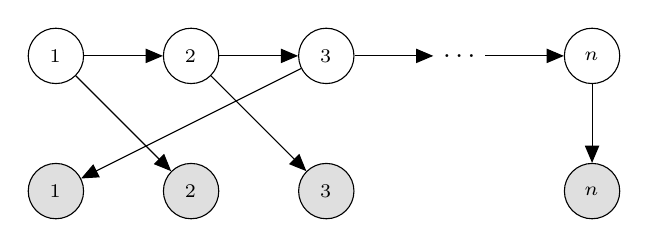
\begin{tikzpicture}
    \node (Ea) [obs] {$\boldx_1$}; 
    \node (Xa) [latent,above =of Ea] {$\boldy_1$}; 

    \node (Eb) [obs, right = of Ea ] {$\boldx_2$}; 
    \node (Xb) [latent,above =of Eb] {$\boldy_2$}; 

    \node (Ec) [obs, right = of Eb] {$\boldx_3$}; 
    \node (Xc) [latent,above =of Ec] {$\boldy_3$}; 
    \node (Xd) [right =of Xc] {$\ldots$}; 
    \node (Xe) [latent,right =of Xd] {$\boldy_n$}; 
    \node (Ee) [obs,below =of Xe] {$\boldx_n$}; 

    \edge {Xa} {Xb} ; %
    \edge {Xb} {Xc} ; %
    \edge {Xa} {Eb} ; %
    \edge {Xb} {Ec} ; %
    \edge {Xc} {Ea} ; %
    \edge {Xc} {Xd} ; %
    \edge {Xd} {Xe} ; %
    \edge {Xe} {Ee} ; %
  \end{tikzpicture}}
\end{center}  

  \end{itemize}
\end{frame}

\begin{frame}{Answer}
  \begin{itemize}
  \item In order time is $O(|\mcW|^2)$. (But exact still intractable).
    \air  

  \item Finding optimal translation is NP-Hard!
    \air 

  \item Reduction from TSP:
    \begin{enumerate}
    \item Each city becomes a source word with a single translation word.
    \item Distance between cities is a bigram LM score $p(w^t_i | w^t_{i-1})$ between words.
    \item A tour is a complete translation (each word used = each city visited)
    \end{enumerate}
  \end{itemize}
\end{frame}

\begin{frame}{How do you find answer?}
  \[  \prod_{i=1}^n p(\boldx_{a_i} | \boldy_i=w^t_i) p(\boldy_i=w^t_i | \boldy_{i-1}=w^t_{i-1}) p(a_i = c_i | a_{i-1}=c_{i-1}, i) \] 

  With constraint that $c_i$ uses each word once.  

  \begin{itemize}
  \item 
  \end{itemize}
\end{frame}

\begin{frame}{Bit-Set Beam Search}
  [Describe on board] 
\end{frame}


\section{Other Details}

\begin{frame}{Training the Translation Model}
  \[ p(w^t | w^s) \] 
  How do you estimate this score? 
\end{frame}


\begin{frame}{MOSES}
  [Show Intro]
\end{frame}

\begin{frame}{More Statistical Machine Translation}
  \begin{itemize}
  \item Handling Length Issues
  \item Producing and Symmetrizing Alignments
  \item Tuning Systems and MERT 
  \item Rare and Unseen Words
  \item Syntactic Translation
  \end{itemize}
\end{frame}

\end{document}